%----------------------------------------------------------------------------------------
%	PACKAGES AND OTHER DOCUMENT CONFIGURATIONS
%----------------------------------------------------------------------------------------

\documentclass[12pt]{report}
\usepackage{polski}
\usepackage[polish]{babel}
\usepackage[utf8]{inputenc}
\usepackage{datetime}
\usepackage{graphicx}

\usepackage{tikz}
\usepackage{amsmath}
\usepackage{multirow}
\usepackage{tabularx}
\usepackage{geometry}
\usepackage{subcaption}
\usepackage{epstopdf}
\usepackage{float}

\geometry{
 	a4paper, 
 	left    = 20mm,
 	right	  = 20mm,
 	top     = 20mm,
 	bottom  = 20mm,
}
 
%----------------------------------------------------------------------------------------
 
%----------------------------------------------------------------------------------------
% DATES
%----------------------------------------------------------------------------------------

\renewcommand{\dateseparator}{.}
\newdate{exercise_date}{15}{12}{2016}


% dodatkowe typy kolumn tabel

% flush left fixed width:
\newcolumntype{L}[1]{>{\raggedright\arraybackslash}p{#1}}

% center fixed width:
\newcolumntype{C}[1]{>{\centering\arraybackslash}p{#1}}

% flush right fixed width:
\newcolumntype{R}[1]{>{\raggedleft\arraybackslash}p{#1}}

%----------------------------------------------------------------------------------------

%----------------------------------------------------------------------------------------
% TIKZ PACKAGES
%----------------------------------------------------------------------------------------

\usetikzlibrary{arrows}

%----------------------------------------------------------------------------------------

\begin{document}
  
\begin{titlepage}

\newcommand{\HRule}{\rule{\linewidth}{0.5mm}}
% Defines a new command for the horizontal lines, change thickness here

\center
% Center everything on the page
 
%----------------------------------------------------------------------------------------
%	LOGO SECTION
%----------------------------------------------------------------------------------------


\includegraphics[width=6cm]{img/logo.png}\\[1cm]
% Include a department/university logo - this will require the graphicx package
 
%----------------------------------------------------------------------------------------
 
%----------------------------------------------------------------------------------------
%	HEADING SECTIONS
%----------------------------------------------------------------------------------------

\textsc{\LARGE Akademia Górniczo-Hutnicza \\[0.2cm]
im. Stanisława Staszica w Krakowie}\\[1.5cm]
% Name of your university/college

\textsc{\Large Elektroniczne systemy diagnostyki medycznej i terapii}\\[0.5cm]
% Major heading such as course name

%----------------------------------------------------------------------------------------
%	TITLE SECTION
%----------------------------------------------------------------------------------------

\HRule \\[0.5cm]
{ \huge \bfseries Klasyfikacja sygnału EKG z wykorzystaniem algorytmów kNN i eNN}\\[0.3cm]
% Title of your document
\HRule \\[1.5cm]

\flushright
\Large \emph{Autorzy:}\\
Wojciech \textsc{Gumuła}\\[0.1cm]
Krzysztof \textsc{Mazur}\\[3cm]
% Authors

%----------------------------------------------------------------------------------------
%	DATE SECTION
%----------------------------------------------------------------------------------------
% Data wykonania ćwiczenia: \\
%{\large \displaydate{exercise_date}}\\[1cm]


\vfill % Fill the rest of the page with whitespace

\end{titlepage}
\section*{Abstrakt}

Celem projektu było zbadanie możliwości wykorzystania algorytmu k-Nearest Neighbours oraz jego rozszerzonej wersji w zadaniu klasyfikacji zespołów \textit{QRS} sygnału \textit{EKG}. Metoda \textit{kNN} charakteryzuje się stosunkowo niewielką złożonością obliczeniową i prostotą implementacji, oferując przy tym klasyfikację z dużą dokładnością. Rozszerzona metoda \textit{eNN} pozwala na uwzględnienie otoczenia klasyfikowanego wektora, co może zwiększyć dokładność wyniku. W ramach projektu przygotowano prototyp algorytmów w środowisku Matlab oraz ich implementację w języku C++ przy użyciu biblioteki Eigen.


\textbf{Słowa kluczowe}:
EKG, QRS, kNN, eNN, klasyfikacja, rozpoznawanie wzorców, Matlab, Eigen.
\tableofcontents

\chapter{Wprowadzenie}
Badanie elektrokardiograficzne, dzięki swej dostępności i łatwości wykonania stanowi jedno z najczęściej wykorzystywanych metod rozpoznawania zaburzeń w pracy serca. Uzyskiwany przy jego pomocy sygnał EKG dostarcza informacji o elektrycznej aktywności mięśnia sercowego, jako różnicę potencjałów pomiędzy dwoma elektrodami.

Jednym z najbardziej charakterystycznych elementów typowego sygnału EKG są zespoły QRS. Jest to układ trzech załamków opisujących proces depolaryzacji mięśnia. Ideowy schemat EKG, wraz z kompleksem QRS przedstawiono na rysunku \ref{fig:qrs-complex}.


\begin{figure}[H]
	\centering
	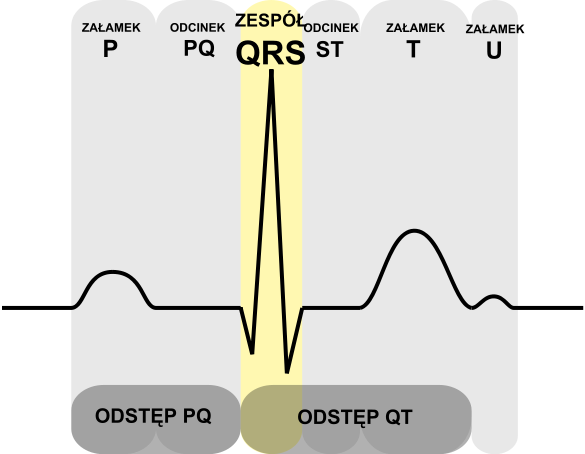
\includegraphics[width=8cm]{img/qrs-complex}
	\caption{Ideowy schemat sygnału EKG. Źródło: \cite{qrs-wiki}}
	\label{fig:qrs-complex}
\end{figure}

Na podstawie charakteru zespołu QRS diagnozować można szereg dysfunkcji serca. Wykorzystanie w tym celu zautomatyzowanych procedur diagnostycznych pozwala na zwiększenie prawdopodobieństwa wykrycia nieprawidłowości i przyśpiesza proces badania. Wymaga to jednak wyodrębnienia grup kompleksów o podobnych parametrów. Uzyskane grupy powinny w odwzorowywać najczęściej występujące zaburzenia pracy.

\section{Koncepcja proponowanego rozwiązanie}

Autorzy badali możliwość wykorzystania algorytmu kNN (\textit{k Nearest Neighbours}) oraz jego rozszerzonej wersji, eNN (\textit{extended Nearest Neighbours}) do zaprojektowania zautomatyzowanego procesu klasyfikacji zespołów QRS do predefiniowanych grup. Opis algorytmów przedstawiono w rozdziałach \ref{chap:knn} i \ref{chap:enn}.

Metody klasy \textit{NN} wymagają przedstawienia danych wejściowych w postaci wektora cech o ustalonym wymiarze. Zdecydowano się wykorzystać w tym celu dane dostępne w opracowaniu \cite{heart-class-module}. Uwzględniono przy tym klasyfikację w zbiorze trzech klas, zaproponowaną przez autorów, a także w zbiorze uwzględniającym wszystkie klasy definiowane w dokumentacji bazy \textit{MIT-BIH} \cite{mitdb}.

Dane wejściowe opisywane są wektorem składającym się z osiemnastu cech. Wektor zawiera informacje na temat chwil wystąpienia kolejnych elementów kompleksu QRS a także wartości sygnału w istotnych chwilach. Jedna z kolumn - chwila wystąpienia załamka R - związana jest jednoznacznie z badanym sygnałem EKG i nie pozwala na klasyfikację w uogólnionym zbiorze danych, z tego powodu jest ignorowana w zaprojektowanym rozwiązaniu.

Celem projektu było zaprojektowanie prototypu proponowanego rozwiązania przy użyciu oprogramowania \textit{Matlab}, a także zgodnej z nim implementacji w języku \textit{C++}. Wykorzystano również bibliotekę \textit{Eigen} \cite{eigen-www}, pozwalającą na optymalizację operacji matematycznych na macierzach i wektorach.

Cykl działania aplikacji podzielić można na dwa etapy.
\begin{enumerate}
	\item Proces uczenia.
	
	Program uczony jest przy użyciu wybranego zbioru danych wejściowych wraz z poprawną klasyfikacją każdego wektora. Dane te są zapamiętywane i wykorzystywane w kolejnym etapie pracy.
	
	\item
	Klasyfikacja danych wejściowych.
	
	Aplikacja pozwala na klasyfikację dowolnej liczby wektorów danych, porównując je z posiadanym zbiorem referencyjnym. Wyjściem programu na wejście zawierające jeden wektor testowy jest klasa, do której został on przypisany.
\end{enumerate}

Test poprawności działania implementacji wymagał podzielenia znanego zbioru danych na podzbiory - uczący i testowy, wraz ze związanymi z nimi klasami. Przyjęto podział w stosunku dwa do jednego. Działanie algorytmu badane było niezależnie dla każdego pliku wejściowego.

\section{Dane wejściowe}
Na etapie testowania działania proponowanych algorytmów wykorzystano dane zgromadzone w ramach biblioteki arytmii pracy serca \textit{MIT-BIH}. Zbiór zawiera czterdzieści osiem zapisów trzydziestominutowych badań \textit{EKG}. Dwadzieścia trzy nagrania stanowią losowo wybrany podzbiór bazy zawierającej zapis kilku tysięcy badań, natomiast pozostałe dwadzieścia pięć nagrań to zbiór dobrany w taki sposób, by zawierał istotne lecz rzadziej występujące klasy arytmii. Dane zawarte w bazie zawierają również precyzyjną klasyfikację kompleksów \textit{QRS} dla każdego nagrania.

Dane zawarte w bazie danych nie mogą być bezpośrednio wykorzystane do przeprowadzenia procesu klasyfikacji. Sygnał wejściowy musi zostać poddany filtracji oraz ograniczony do wektorów cech opisujących kolejne zespoły \textit{QRS}. W ramach projektu wykorzystano wstępnie przygotowane dane wejściowe, zawierające wektory cech i adnotacje klas.

Wykorzystując opisany zbiór wejściowy, badano skuteczność detekcji klas przez algorytm. Sprawdzano również możliwość zaprojektowania zbioru uczącego w taki sposób, aby jak najlepiej reprezentował on klasy sygnału, maksymalizując skuteczność detekcji w zbiorze zawierającym wszystkie pliki danych.
\section{Algorytm kNN}
\label{chap:knn}
Algorytm kNN (ang. \textit{k Nearest Neighbours})  jest jednym z najprostszych algorytmów klasyfikacyjnych, należy również do najpopularniejszych ze względu na prostotę implementacji oraz dobre wyniki obliczeń. Reguła klasyfikacji opiera się na założeniu, że dane przedstawione w $n$-wymiarowej przestrzeni zgrupowane będą w obszarach opisanych podobnymi cechami. Bazując na tym założeniu, ustalenie klasy dla wektora wejściowego sprowadza się do zbadania jego najbliższego otoczenia w przestrzeni i wyboru klasy najczęściej w nim występującej.

Pierwszym krokiem algorytmu jest wyznaczenie odległości pomiędzy próbką ze zbioru testowego, oraz wszystkimi próbkami ze zbioru uczącego. Najczęściej stosowaną metodą wyznaczania odległości jest metryka euklidesowa dana poniższym wzorem, gdzie $N$ to szerokość wektora dla każdej próbki:

\begin{equation}
d(x,y) = \sum_{i=1}^{N} \sqrt{(x_i - y_i)^2}.
\end{equation}

Następnie ze zbioru $K$ najbliższych sąsiadów wybierana jest najczęściej występująca klasa obiektów, a rozważany przypadek klasyfikowany jest jako obiekt tej klasy. Dobór optymalnego parametru $K$ odbywa się zazwyczaj na drodze eksperymentów stosując nieparzyste wartości $K=1,3,5...$ . Proces uczenia jest bardzo prosty i ogranicza się do zapamiętania wszystkich próbek ze zbioru uczącego. Konieczność wyznaczenia odległości pomiędzy klasyfikowaną próbką a wszystkimi próbkami ze zbioru uczącego wymusza rozważne przygotowanie tego ostatniego. Zawarte w nim wartości powinny dobrze definiować całą przestrzeń, jednocześnie minimalizując rozmiar w celu przyspieszenia działania algorytmu. Poza klasyfikacją algorytm kNN wykorzystywany jest także do klasteryzacji, regresji, estymowania funkcji gęstości. W 2006 roku algorytm został zaliczony do 10 najpopularniejszych algorytmów w dziedzinie eksploracji danych podczas konferencji IEEE w Hong Kongu.

Zasadę działania algorytmu na przykładzie przedstawiono na rysunku \ref{fig:knn-idea}.

\begin{figure}[H]
	\centering
	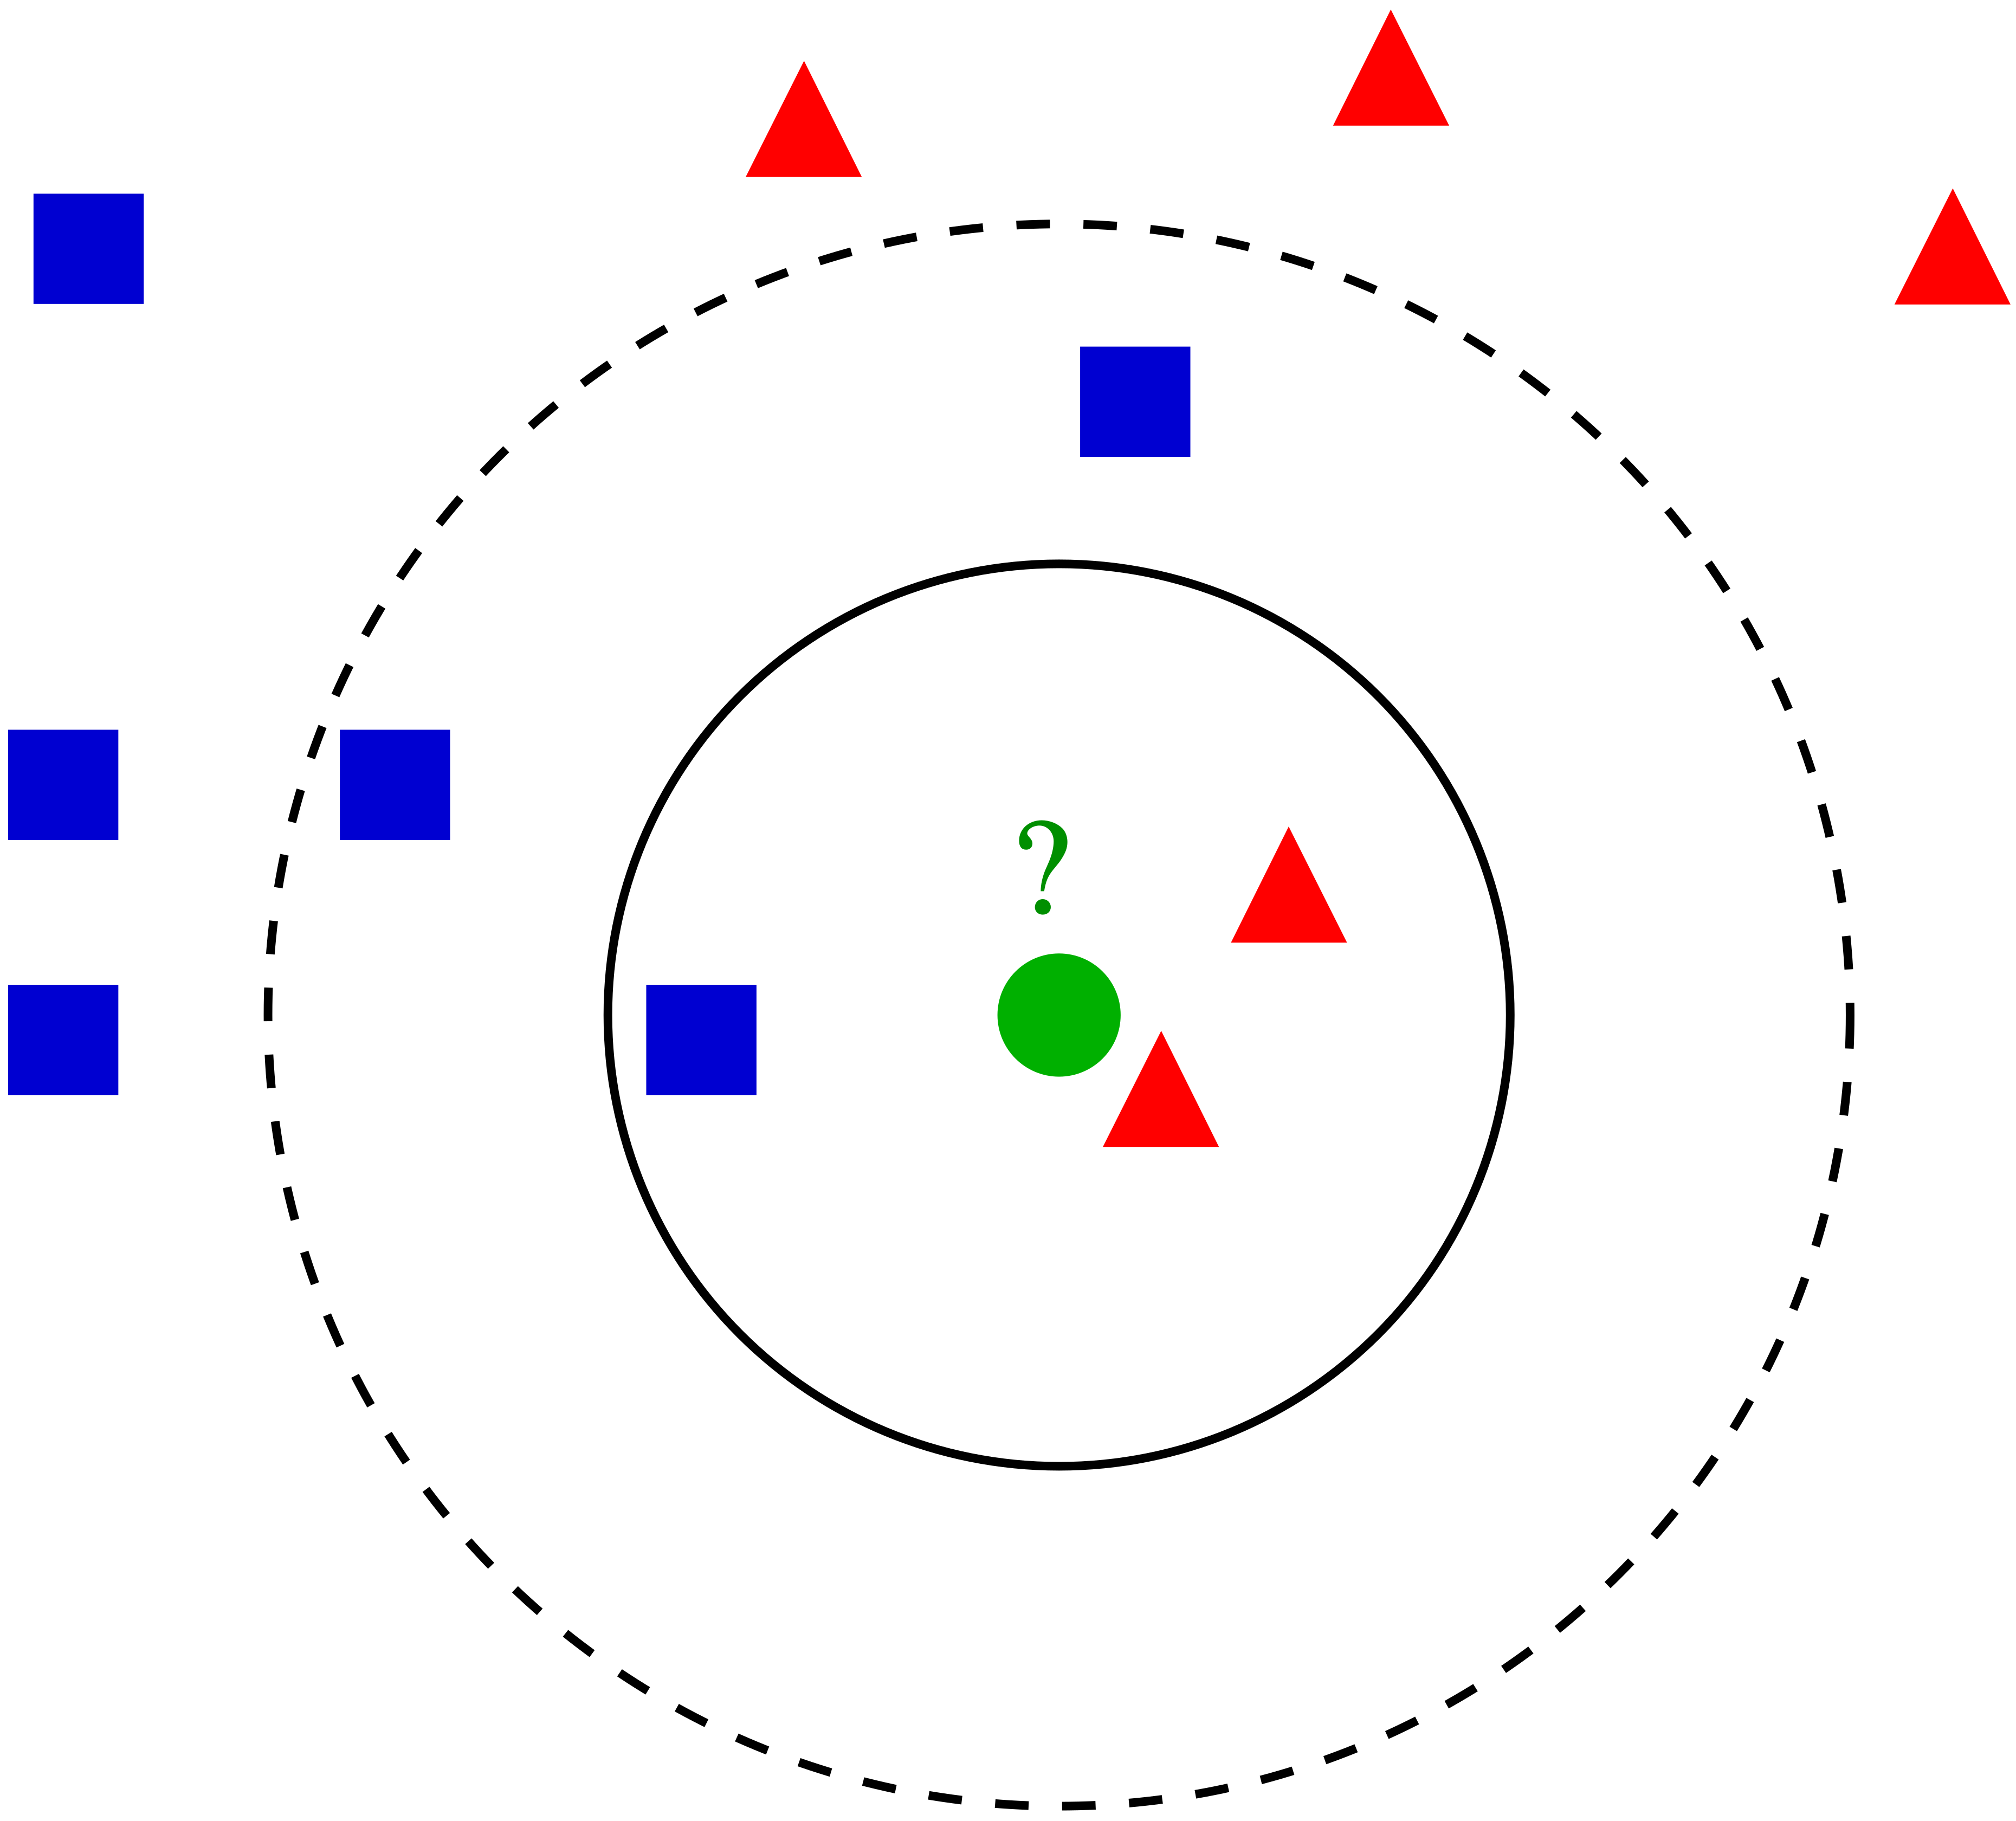
\includegraphics[width=10cm]{img/KnnClassification}
	\caption{Schematyczne przedstawienie klasyfikacji dwuwymiarowego wektora danych. Źródło \cite{knn-wiki}}
	\label{fig:knn-idea}
\end{figure}

Zadaniem klasyfikacji jest ustalenie przynależności wartości wejściowej - koła, do jednej z dwóch grup elementów - kwadratów i trójkątów. Przyjmując wartość parametru $K=3$ (linia ciągła na rysunku), wartość przypisana zostanie do grupy zawierającej trójkąty. Zakładając $K=5$ wynik będzie przeciwny i element zostanie powiązany z grupą zawierającą kwadraty.

Dobór wartości parametru $K$ dającej najlepsze wyniki wymaga więc znajomości badanego zjawiska bądź przeprowadzenia doświadczeń na reprezentatywnym zbiorze testowym.

\chapter{Algorytm eNN}
\label{chap:enn}
\section{Podstawowa wersja algorytmu}
\large{Algorytm kNN pomimo wielu swoich zalet ma także kilka wad, które w niektórych przypadkach mogą niekorzystnie wpływać na wyniki działania. Jednym z charakterystycznych problemów jest przypadek kiedy rozkłady gęstości poszczególnych klas nie są równe. W takiej sytuacji elementy klasy o większym rozkładzie gęstości przeważają nad elementami pozostałych klas na danym obszarze. Dla algorytmu większość najbliższych sąsiadów będzie pochodziła z dominującej klasy co może zakłócać poprawność działania.

Jako rozwinięcie algorytmu kNN został stworzony algorytm eNN (\textit{ang. Extended Nearest Neighbours}) \cite{haibo-he}. Zaproponowana metoda podczas klasyfikacji bierze pod uwagę nie tylko k najbliższych sąsiadów klasyfikowanego obiektu, ale również ich otoczenie. 

Dla uproszczenia opis algorytmu zostanie przeprowadzony dla przypadku klasyfikacji pomiędzy dwoma klasami. Uogólnienie algorytmu dla dowolnej ilości klas sprowadza się jedynie do większej złożoności obliczeniowej. Dla każdego z k najbliższych sąsiadów próbki ze zbioru testowego wyznaczana jest funkcja statystyczna T opisująca otoczenie w jakim się znajduje. Funkcja T wyznaczana jest według wzoru:

\begin{equation}
T_{i} = \frac{1}{n_i k} {\sum_{x \in S_i} \sum_{r=1}^{k} I_r (x,S \in (S_1 \cup S_2))} 
\end{equation}\\
gdzie $S_1$ i $S_2$ są zbiorami próbek należących odpowiednio do klas 1 i 2, k jest zdefiniowaną ilością najbliższych sąsiadów a $I_r$ dane jest wzorem:

\begin{equation}
I_r(x,S) =\left\{\begin{matrix}
1 &&	dla\ x \in S_i \wedge NN_{r}(x,S) \in S_i
\\
0 &&	w\ pozostałych\ przypadkach
\end{matrix}\right.
\end{equation}
Funkcja $I_r$ przyjmuje wartość 1 jeżeli próbka x i jej r-sąsiad należą do tej samej klasy, natomiast wartość 0 przyjmuje w pozostałych przypadkach.
Funkcja $T_i$ przyjmuje wartości z zakresu [0,1]. Im większa wartość $T_i$ tym więcej próbek tej samej klasy znajduje się w otoczeniu badanej próbki. Małe wartości oznaczają małą ilość próbek tej samej klasy.

Mając nową, niesklasyfikowaną próbkę, w kolejnych krokach zostaje przypisana do poszczególnych klas a następnie dla każdego przypadku wyznaczona zostaje wartość funkcji $T_i^j$ według wzoru:

\begin{equation}
T_{i}^{j} = \frac{1}{n_i^j k} {\sum_{x \in S_{i,j}'} \sum_{r=1}^{k} I_r (x,S' \in (S_1 \cup S_2 \cup {Z}))} 
\end{equation}\\
gdzie j oznacza klasę do której została przypisana próbka Z.
W rozważanym przypadku, gdy pod uwagę brane są dwie klasy otrzymujemy cztery wyniki $T_1^1, T_2^1, T_1^2\ oraz\ T_2^2$. Próbka Z zostaje zakwalifikowana zgodnie ze wzorem:

\begin{equation}
f_{ENN} = arg_{j\in1,2} max \sum_{i=1}^{2} T_i^j
\end{equation}
Powyższy wzór w przypadku gdy w zbiorze znajduje się N klas występuje w postaci:
\begin{equation}
f_{ENN} = arg_{j\in1,2,..,N} max \sum_{i=1}^{N} T_i^j
\end{equation}
Klasyfikacja próbki do odpowiedniej klasy odbywa się poprzez wybór maksymalnej wartości funkcji $T_i$ spośród wyznaczonych metodą iteracyjną wartości dla kolejnych klas.

\newpage
\section{Alternatywna wersja algorytmu}
Analizując podstawową wersję algorytmu eNN można zaobserwować konieczność wyznaczenia wartości $T_i^j$ dla każdej kolejnej klasyfikowanej próbki. Wiąże się to  ze wzrostem złożoności obliczeniowej co nie jest pożądane w przypadku dużych zbiorów testowych. Rozwiązaniem tego problemu jest równoważna wersja algorytmu eNN, która została przedstawiona w tym paragrafie. 

W rozważanej wersji algorytmu pod uwagę brane jest nie tylko kto znajduje się w zbiorze najbliższych sąsiadów klasyfikowanej próbki Z ale także które próbki ze zbioru uczącego biorą pod uwagę próbkę Z jako jednego z k najbliższych sąsiadów. W tym celu próbka Z zostaje przypisana kolejno do wszystkich klas. W każdym przypadku zostają wyznaczone wartości $\Delta n_i^j$ gdzie j jest klasą do której została przypisana próbka Z, natomiast i jest klasą dla której obliczana jest zmiana ilości sąsiadów tej samej klasy. W przypadku gdy i = j zliczana jest ilość próbek klasy i dla której wzrosła ilość sąsiadów należących do tej samej klasy. W przypadku gdy $i\ \neq j$ wyznaczana jest ilość próbek klasy i dla których zmalała ilość sąsiadów należących do tej samej klasy.

Dla wyznaczonych wartości $n_i^j$ klasyfikacja próbki Z realizowana jest zgodnie z zależnością:

\begin{equation}
f_{ENN} = arg_{j \in 1,2,..,N} max \begin{Bmatrix}
(\frac{\Delta n_i^j + k_j -kT_i}{(n_i+1)k})
\end{Bmatrix}_{i=j} - \sum_{i \neq j}^N \frac{\Delta n_i^j}{n_i k}
\end{equation}\\
gdzie k jest zdefiniowaną ilością najbliższych sąsiadów, $n_i$ jest ilością próbek należących do klasy i, a $k_i$ jest ilością najbliższych sąsiadów należących do klasy i.

Obie wersje algorytmu są równoważne, jednak w przypadku drugiej wersji na początku działania algorytmu można wyznaczyć wektor wartości $T_i$ a podczas klasyfikacji kolejnych próbek ograniczyć się do wyznaczenia zmian w otoczeniach k najbliższych sąsiadów próbki Z, dla kolejnych przypisań próbki Z do odpowiednich klas.

\begin{thebibliography}{9}
	\bibitem{haibo-he} 
	Bo Tang i Haibo He. 
	\textit{Enn: Extended Nearest Neighbor Method for Pattern Recognition}. 
	IEEE Computational intelligence magazine. 2015
	
	\bibitem{enn-impl}
	Haibo He.
	\textit{Referencyjna implementacja algorytmu eNN}.
	\\\texttt{http://www.ele.uri.edu/faculty/he/research/ENN/ENN.html}
	
	\bibitem{qrs-wiki}
	Wikipedia.
	\textit{QRS complex}.	\\\texttt{https://en.wikipedia.org/wiki/QRS\_complex}
	
	\bibitem{knn-wiki}
	Wikipedia.
	\textit{k-nearest neighbors algorithm}.	\\\texttt{https://en.wikipedia.org/wiki/K-nearest\_neighbors\_algorithm}
	\bibitem{mitdb}
	\textit{MIT-BIH Arrhythmia Database}.	\\\texttt{https://www.physionet.org/physiobank/database/mitdb/}
	
	\bibitem{heart-class-module} 
	Michał Ciszewski, Łukasz Dudek i Krystian Mucha.
	\textit{Moduł HeartClass}.
	
	\bibitem{eigen-www}
	\textit{Eigen Library}.
	\\\texttt{http://http://eigen.tuxfamily.org/}
\end{thebibliography}

\end{document}